\section{Debugging}\label{section:konzeption:debugging}

Nach \autoref{requirement:Debuggen} soll das Debuggen der Programme von Nutzern innerhalb der IDE ermöglicht werden. Dafür soll laut Unteranforderung (a) ein CrossLab-Service für die Bereitstellung und Nutzung von Debuggern entwickelt werden. Weiterhin verlangt Unteranforderung (b) die Entwicklung eines CrossLab-Service für die Kommunikation zwischen Debuggern und Steuereinheiten. Der aus Unteranforderung (a) resultierende CrossLab-Service soll nach Unteranforderung (b) von der IDE für die Nutzung von Debuggern verwendet werden. Dementsprechend werden im Folgenden der \textit{Debugging Adapter Service} für die Bereitstellung und Nutzung von Debuggern sowie der \textit{Debugging Target Service} für die Kommunikation zwischen Debuggern und Steuereinheiten vorgestellt.

Der Debugging Adapter Service baut auf dem \textit{\ac{DAP}} \cite{noauthor_debug-adapter-protocol_nodate} von Microsoft auf. Dieses spezifiziert Nachrichten, die zwischen einer IDE und einem sogenannten \textit{Debug Adapter} ausgetauscht werden. Ein Debug Adapter bildet die Schnittstelle zwischen einem Debugger und einer IDE. Das Protokoll erlaubt somit die Anbindung bestehender Debugger über die Implementierung eines entsprechenden Debug Adapters. Weiterhin wird der Implementierungsaufwand für die Einbindung von Debuggern in IDEs verringert, da nur eine Schnittstelle implementiert werden muss, anstatt jeden Debugger an eine eigens entwickelte Schnittstelle anpassen zu müssen.

\begin{figure}[tbp]
    \centering
    \resizebox{0.9\textwidth}{!}{\begin{sequencediagram}
            \newthread{ide}{IDE}
            \newthreadShift{debugger}{Debugger}{3cm}
            \newthreadShift{steuereinheit}{Steuereinheit}{3cm}

            \begin{call}{ide}{starte Debug-Sitzung}{debugger}{}
                \begin{call}{debugger}{speichere Programm}{debugger}{}
                \end{call}
                \begin{call}{debugger}{kompiliere Programm}{debugger}{}
                \end{call}
                \begin{call}{debugger}{starte Debuggen}{steuereinheit}{}
                    \begin{call}{steuereinheit}{lade Programm}{steuereinheit}{}
                    \end{call}
                \end{call}
            \end{call}

            \begin{call}{ide}{DAP Nachrichten}{debugger}{DAP Nachrichten}
            \end{call}

            \prelevel\prelevel

            \begin{call}{debugger}{Debugger Nachrichten}{steuereinheit}{Debugger Nachrichten}
            \end{call}
        \end{sequencediagram}}
    \caption{Start einer Debug-Sitzung}
    \label{figure:start-einer-debug-sitzung}
\end{figure}

\paragraph{Start einer Debug-Sitzung} \autoref{figure:start-einer-debug-sitzung} zeigt ein Sequenzdiagramm für den Start einer Debug-Sitzung. Debug-Sitzungen können über Debugging Adapter Service Consumer gestartet werden. Dabei werden der Ordner, welcher das zu debuggende Programm enthält, und dessen URI bzw. Pfad sowie Konfigurationsoptionen für den Debugger an den Debugging Adapter Service Producer gesendet. Der Start einer Debug-Sitzung ist abhängig vom verwendeten Debugger. Im Allgemeinen sollte zunächst der übersendete Ordner auf dem Dateisystem des Debugging Adapter Service Producer gespeichert werden. Weiterhin kann ggf. eine Kompilierung des Programms mit speziellen Optionen für das Debuggen vorgenommen werden. Außerdem sollte der Debugger mit den Konfigurationsoptionen gestartet werden und es sollte ein eindeutiger Kennzeichner für die Debug-Sitzung generiert werden. Darüber hinaus sollte die zu debuggende Steuereinheit über den Start der Debug-Sitzung informiert werden. Dafür wird über den Debugging Target Service Consumer des Debuggers eine entsprechende Nachricht an die Steuereinheit gesendet. Diese enthält das zu debuggende Programm. Dieses kann, wie bereits für den Programming Service in \autoref{section:konzeption:kompilierung-und-programmierung} beschrieben, eine Datei oder ein Ordner sein. Das Programm kann z.B. zur Programmierung der Steuereinheit verwendet werden. Zusätzlich können ggf. noch weitere Vorbereitungen getroffen werden, bevor eine Antwort an den Debugging Target Service Consumer gesendet wird. Nachdem die Sitzung erfolgreich gestartet wurde, wird eine entsprechende Antwort an den Debugging Adapter Service Consumer gesendet. Diese enthält den Kennzeicher der Debug-Sitzung sowie weitere Konfigurationsoptionen, die beim Start des \ac{DAP} übergeben werden sollen. Bei diesen Konfigurationsoptionen handelt es sich um Informationen, die nur dem Debugging Adapter Service Producer bekannt sind, wie z.B. der Pfad zu dem kompilierten Programm auf dessen Dateisystem. Sobald der Debugging Adapter Service Consumer die Antwort erhalten hat, kann das \ac{DAP} mit den Konfigurationsoptionen und dem Kennzeichner der Debug-Sitzung gestartet werden. Die in DAP Nachrichten enthaltenen URIs müssen für den Debug Adapter bzw. die IDE angepasst werden, da diese auf unterschiedlichen Dateisystemen arbeiten. Die Kommunikation zwischen dem Debugger und der Steuereinheit erfolgt über den Debugging Target Service.

\begin{figure}[tbp]
    \centering
    \resizebox{0.9\textwidth}{!}{\begin{sequencediagram}
            \newthread{ide}{IDE}
            \newthreadShift{debugger}{Debugger}{4cm}
            \newthreadShift{steuereinheit}{Steuereinheit}{3cm}

            \begin{call}{ide}{DAP Terminate Anfrage}{debugger}{}
                \begin{call}{debugger}{lösche Sitzungsdaten}{debugger}{}
                \end{call}
                \begin{call}{debugger}{stoppe Debugger}{debugger}{}
                \end{call}
                \begin{call}{debugger}{beende Debuggen}{steuereinheit}{}
                    \begin{call}{steuereinheit}{lade Programm neu}{steuereinheit}{}
                    \end{call}
                \end{call}
            \end{call}
        \end{sequencediagram}}
    \caption{Ende einer Debug-Sitzung}
    \label{figure:ende-einer-debug-sitzung}
\end{figure}

\paragraph{Ende einer Debug-Sitzung} \autoref{figure:ende-einer-debug-sitzung} zeigt ein Sequenzdiagramm für das Ende einer Debug-Sitzung. Dieses wird durch eine entsprechende Nachricht des \ac{DAP} wie z.B. \texttt{Terminate} ausgelöst. Sobald der Debug Adapter diese Nachricht erhält, werden die Sitzungsdaten gelöscht und der Debugger gestoppt. Weiterhin wird vom Debugging Target Service Consumer eine Nachricht an den Debugging Target Service Producer gesendet, um diesen über das Ende der Debug-Sitzung zu informieren. Dieser kann dann z.B. das aktuelle Programm neuladen und weitere vorgenommene Änderungen für das Debuggen rückgängig machen. Danach wird eine entsprechende Antwort an den Debugging Target Service Consumer gesendet. Sobald diese erhalten wurde, wird noch eine finale Antwort auf die ursprüngliche \ac{DAP} Anfrage gesendet.

\paragraph{Kollaboration} Nach \autoref{requirement:Teilen von Debug-Sitzungen} soll es Nutzern innerhalb eines Experiments ermöglicht werden, laufenden Debug-Sitzungen beizutreten. Dafür soll laut Unteranforderung (e) der bereits vorhandene Collaboration Service der IDE verwendet werden. Über diesen könnten z.B. beim Start einer Debug-Sitzung der Kennzeichner der Sitzung und der verwendete Ordner in den Zustandsinformationen des Nutzers hinterlegt werden. Dadurch können andere Nutzer über die gestartete Sitzung informiert werden. Falls sie Zugriff auf den angegebenen Ordner haben, können sie der Debug-Sitzung mithilfe des Debugging Adapter Service Consumer beitreten. Dabei wird der Kennzeichner der beizutretenden Debug-Sitzung angegeben. Die Antwort enthält einen neuen Kennzeichner für die Debug-Sitzung des beitretenden Nutzers sowie Konfigurationsoptionen für die Ausführung des \ac{DAP}. Um eine kollaborative Debug-Sitzung zu ermöglichen, ist zudem eine spezielle Behandlung von einigen Nachrichten des \ac{DAP} nötig. Zum Beispiel darf nur eine \texttt{Initialize} Anfrage an einen Debug Adapter gestellt werden. Dementsprechend muss die Antwort auf diese gespeichert werden, um sie später bei einer erneuten \texttt{Initialize} Anfrage an den beitretenden Nutzer senden zu können. Dabei wird die Anfrage beitretender Nutzer nicht an den Debug Adapter übergeben. Weiterhin sind z.B. die Nachrichten für Breakpoints, Stacktraces, das Starten und Stoppen des Programms sowie das Beenden der Debug-Sitzung zu betrachten. Die detaillierte Betrachtung aller dieser Nachrichten ist nicht das Ziel dieser Arbeit. In \autoref{section:prototypische-implementierung:debugging} wird die Behandlung der Nachrichten erläutert, welche für die prototypische Implementierung relevant sind.

Die betrachtete Experimentkonfiguration wird zunächst um ein Laborgerät erweitert. Dieses stellt einen Debugger über einen entsprechenden Debugging Adapter Service Producer bereit. Weiterhin besitzt dieses noch einen Debugging Target Service Consumer zur Kommunikation mit der zu debuggenden Steuereinheit. Die IDE wird um einen Debugging Adapter Service Consumer erweitert. Die Steuereinheit wird um einen Debugging Target Service Producer erweitert. Das neue Laborgerät wird über die entsprechenden CrossLab-Services mit der IDE und der Steuereinheit verbunden. Die Erweiterung der betrachteten Experimentkonfiguration ist in \autoref{figure:experimentkonfiguration:debugging} dargestellt.

\begin{figure}[tbp]
    \centering
    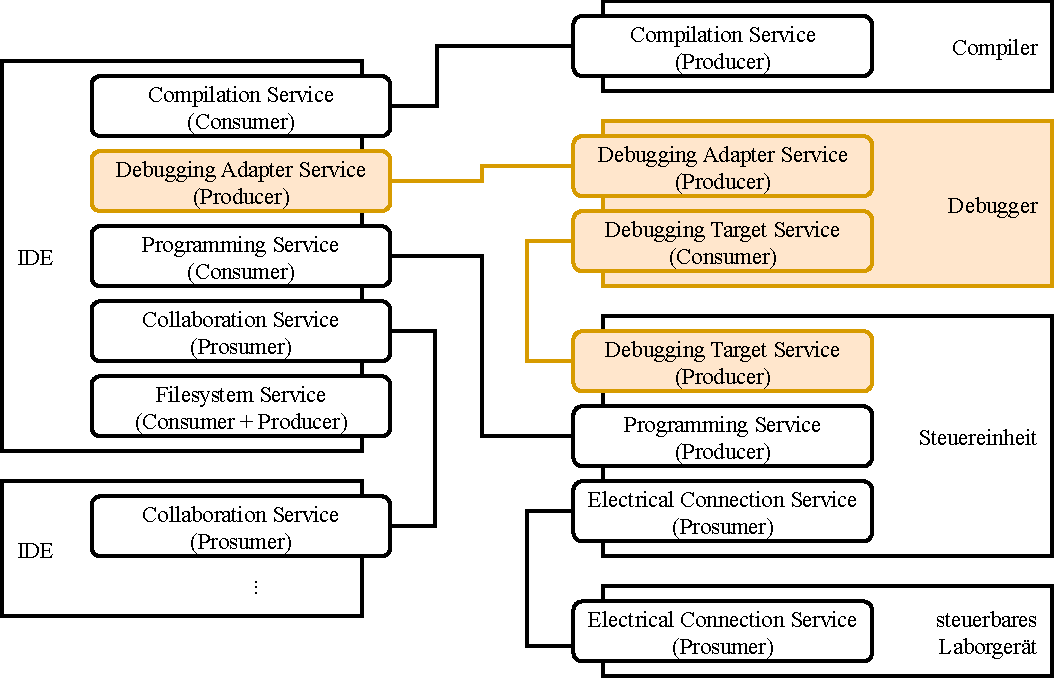
\includegraphics[width=\textwidth]{diagrams/experimentkonfigurationen/Experimentkonfiguration-04.drawio.pdf}
    \caption{Experimentkonfiguration (+ Debugging)}
    \label{figure:experimentkonfiguration:debugging}
\end{figure}